\begin{enumerate}
\item
 \begin{enumerate}
 \item Pour $z$ dans $\mathcal{H}$, calculons la partie imaginaire de
\begin{displaymath}
 \frac{z\cos\theta-\sin\theta}{z\sin\theta+\cos\theta}
\end{displaymath}
en multipliant le numérateur et le dénominateur par le conjugué $\bar{z}\sin \theta + \cos \theta$ du dénominateur. Après développement du numérateur, on trouve :
\begin{displaymath}
 \frac{\Im (z)}{|z\sin\theta+\cos\theta|^2}
\end{displaymath}
qui est bien strictement positif pour $z$ dans $\mathcal{H}$.
\item Vérifions les formules demandées
\begin{displaymath}
 \forall z\in \mathcal{H},
A_0(z) = \frac{z\cos 0 - \sin 0}{z\ sin 0 + \cos 0}=z
\end{displaymath}
Comme ceci est valable pour tous les $z$ de $\mathcal{H}$, on a bien $A_0= \Id_\mathcal{H}$.\newline
De même
\begin{multline*}
\forall z\in \mathcal{H}, A_\theta \circ A_{\theta'}(z)
=\frac
{\frac{z\cos \theta' - \sin \theta'}{z\sin\theta' + \cos \theta'}\cos \theta - \sin \theta}
{\frac{z\cos \theta' - \sin \theta'}{z\sin\theta' + \cos \theta'}\sin\theta + \cos \theta} \\
=\frac
  {z(\cos\theta' \cos\theta - \sin\theta' \sin \theta) -\sin\theta' \cos \theta - \cos \theta'\sin\theta }
  {z(\cos \theta' \sin \theta + \sin \theta' \cos \theta) -\sin\theta'\sin\theta + \cos\theta'\cos \theta}\\
= \frac{z \cos(\theta + \theta')-\sin(\theta + \theta')}{z\sin(\theta + \theta')+\cos(\theta + \theta')}
= A_{\theta + \theta'}(z)
\end{multline*}
Comme ceci est valable pour tous les $z$ de $\mathcal{H}$, on a bien $A_\theta \circ A_\theta' = A_{\theta + \theta'}$.\newline
Pour montrer la bijectivit{\'e} de $A_\theta$, on doit prouver que: pour tout $Z$ de $\mathcal{H}$, il existe un unique ant{\'e}c{\'e}dent $z\in \mathcal{H}$ tel que $A_\theta(z) = Z$.\newline
Une première méthode consiste à combiner le raisonnement par analyse-synthèse avec les résultats des questions précédentes.\newline
Analyse.\newline
Soit $z \in \mathcal{H}$ tel que $Z=A_\theta(z)$. Alors en composant par $A_{-\theta}$:
\begin{displaymath}
  A_{-\theta}(Z) = A_{-\theta}\circ A_{\theta}(z) = A_{-\theta + \theta}(z) = A_0(z) = Id_{\mathcal{H}}(z)=z
\end{displaymath}
Ceci assure l'unicité de $z$ c'est à dire l'injectivité de $A_\theta$. Le seul $z$ éventuellement possible est $A_{-\theta}(Z)$.\newline
Synthèse.\newline
Vérifions que $A_{-\theta}(Z)$ satisfait bien à la condition requise.\newline
D'abord, il est dans $\mathcal{H}$ car toutes les images par $A_{-\theta}$ sont dans $\mathcal{H}$. Ensuite:
\begin{displaymath}
  A_\theta\left( A_{-\theta}(Z)\right) = A_{\theta - \theta}(Z) = Z
\end{displaymath}
Ceci achève de montrer la partie \og existence\fg~ de la proposition cette partie correspond à la surjectivité de l'application.\newline
Si on ne pense pas à la solution précédente, on peut présenter la rédaction de la manière suivante.
{\'E}tudions l'{\'e}quation $A_\theta (z)=Z$. Il s'agit en fait d'une équation du premier degré. Apr{\`e}s calculs, on trouve
\begin{displaymath}
 A_\theta (z)=Z\Leftrightarrow z=\frac{Z\cos \theta + \sin \theta}{-Z \sin \theta + \cos \theta}
\end{displaymath}
Le d{\'e}nominateur n'est pas nul car $Z$ n'est pas r{\'e}el. Ceci prouve l'injectivit{\'e} de $A_\theta$. Chaque $Z$ admet au plus un ant{\'e}c{\'e}dent, le seul possible est
\begin{displaymath}
 \frac{Z\cos \theta + \sin \theta}{-Z \sin \theta + \cos \theta}
\end{displaymath}
Mais ce nombre est-il bien un {\'e}l{\'e}ment de $\mathcal{H}$? En fait oui car il s'{\'e}crit $A_{-\theta}(Z)$ et il est dans $\mathcal{H}$ {\`a} cause de la question a. Ceci prouve la
bijectivit{\'e}. Remarquons que $A_{-\theta}=A_\theta ^{-1}$.
\end{enumerate}

\item
 \begin{enumerate}
 \item  Sans chercher {\`a} pr{\'e}ciser les parties r{\'e}elles et imaginaires de $A_\theta (z)$, on peut {\'e}crire
\begin{displaymath}
 |A_\theta (z)|^2+1 = 
\frac{|z\cos\theta-\sin\theta|^2+|z\sin\theta+\cos\theta|^2}
     {|z\sin\theta+\cos\theta|^2}=\frac{|z|^2+1}{|z\sin\theta+\cos\theta|^2}
\end{displaymath}
en utilisant deux fois la formule exprimant le carré du module d'une somme. 
Introduisons ensuite la valeur de $\Im (A_\theta (z))$ trouv{\'e}e en 1.a. On obtient finalement
\begin{displaymath}
 c(A_\theta (z))= \frac{|z|^2+1}{|z\sin\theta+\cos\theta|^2} \, \frac{|z\sin\theta+\cos\theta|^2}{\Im (z)} = c(z)
\end{displaymath}
\item Pour $z\neq i$ dans $\mathcal{H}$, comme $z^2+1\neq0$, les {\'e}galit{\'e}s suivantes sont {\'e}quivalentes
\begin{multline*}
\frac{z\cos\theta-\sin\theta}{z\sin\theta+\cos\theta} = 
     \frac{z\cos\theta^{\prime}-\sin\theta^{\prime}}{z\sin\theta^{\prime}+\cos\theta^{\prime}}\\
\Leftrightarrow    z^2\cos \theta \sin \theta^{\prime}-\sin \theta \cos \theta^{\prime} =
    z^2\sin \theta \cos \theta^{\prime}-\cos \theta \sin \theta^{\prime} \\
\Leftrightarrow    (z^2+1) \sin(\theta - \theta^{\prime}) = 0
\Leftrightarrow \theta \equiv \theta' \mod \pi
\end{multline*}
   \end{enumerate}

\item
\begin{enumerate}
\item Consid{\'e}rons un $z_0$ dans $\mathcal{H}-\{i\}$, et posons $k_0=c(z_0)$. Remarquons que c'est un réel strictement positif.\newline
Montrons que tout élément $z$ de $\mathcal{O}$ est dans $\mathcal{C}_{z_0}$.\newline
Par définition de $\mathcal{O}$, il existe $\theta \in \R$ tel que $z=A_\theta(z_0)$. Ceci entraine en particulier que la partie imaginaire de $z$ est strictement positive. Calculons $|z-ic(z_0)|$ ou plutôt son carré.
\begin{multline*}
 |z-ic(z_0)|^2 = |z|^2 +2k_0\Re(iz)+k_0^2= |z|^2 -2k_0\Im(z)+k_0^2\\
= |z|^2+1 -2k_0\Im(z) + k_0^2 -1 
= 2\Im(z)c(z) -2k_0\Im(z) + k_0^2 -1 \\
= (c(z)-k_0)2\Im(z)+k_0^2-1
\end{multline*}
Or d'après 2.a. $c(z)=c(z_0)=k_0$ donc
\begin{displaymath}
 |z-ic(z_0)|^2 = k_0^2-1
\end{displaymath}
On en déduit que $z$ est sur le cercle $\mathcal{C}_{z_0}$.
\begin{figure}
      \centering
      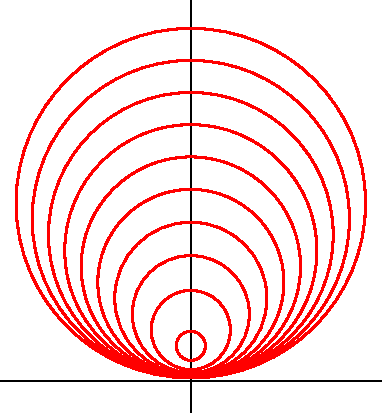
\includegraphics{CpPoinc_1.pdf}
      \caption{Question 3.b. : tracé de quelques cercles $\mathcal{C}(z_0)$}
      \label{CpPoinc_1}
\end{figure}

\item Pour fixer les id{\'e}es tra\c{c}ons (figure \ref{CpPoinc_1}) quelques cercles $\mathcal{C}_{z_0}$ pour des valeurs $z_0$ particulières. Il s'agit de montrer que \emph{tous} les points d'un $\mathcal{C}_{z_0}$ sont sur $\mathcal{O}$.\newline
Pour all{\'e}ger les notations, je vais utiliser $z$ au lieu de $z_0$. On va montrer que tout $z'\neq z$ de $\mathcal{C}_z$ est de la forme $A_{\theta}(z)$ pour un certain $\theta \in ]0,\pi[ $.\newline
Or $A_{\theta}(z)=z'$ est {\'e}quivalent {\`a}
\begin{displaymath}
 \frac{z\cos \theta - \sin\theta}{z\sin \theta + \cos \theta} = z'
 \Leftrightarrow
 \frac{z\cotan \theta -1}{z + \cotan \theta} = z'
 \Leftrightarrow
 \cotan \theta=\frac{1+zz'}{z-z'}
\end{displaymath}
On montre {\`a} partir des propri{\'e}t{\'e}s de $\tan$ que la fonction cotangente d{\'e}finit une bijection de $]0,\pi[$ sur
$\R$. Pour montrer l'existence d'un $\theta$, il suffit donc de prouver que
\begin{displaymath}
 \frac{1+zz'}{z-z'}
\end{displaymath}
est r{\'e}el lorsque $z'\in\mathcal{C}_z$.\newline Cela r{\'e}sulte des {\'e}quivalences suivantes :
\begin{multline*}
z'\in\mathcal{C}_z \Leftrightarrow 
c(z')=c(z) \Leftrightarrow \frac{|z|^2+1}{z-\bar{z}}=\frac{|z'|^2+1}{z'-\bar{z'}} \\
 \Leftrightarrow 
|z|^2z'+z'-|z|^2\bar{z'}-\bar{z'}=z|z'|^2+z-\bar{z}|z'|^2-\bar{z}\\
\Leftrightarrow
\bar{z}+|z|^2\bar{z'}-\bar{z'}-z|z'|^2=z+|z|^2\bar{z'}-z'-\bar{z}|z'|^2\\
\Leftrightarrow
\bar{z}+|z|^2\bar{z'}-\bar{z'}-z|z'|^2 \in \R
 \Leftrightarrow  (1+zz')(\bar{z}-\bar{z'})\in \R
 \Leftrightarrow  \frac{1+zz'}{z-z'}\in \R
\end{multline*}
   \end{enumerate}
\end{enumerate}